\subsubsection{Parser: parse LLVM IR to Module insts}

The detailed process is as follows:
    \begin{itemize}
        \item IR parsing

IR is composed of the following structure: module -> function -> value -> types.

(1) Module structure contains Target (triple and datalayout information), Function, Attribute, and GlobalVariable.

(2) Function structure contains name, type information, Visibility, Attribute and Parameter list basic information, and data, Layout.

(3) Among them, layout contains the sequential logical relationship between basicBlocks and the instructions within them.

(4) Data contains the specific Value, Instruction, BasicBlock list instances.

(5) BasicBlock is identified by BasicBlockId and consists of two parts: name and number. Each BB block usually contains one preds and one sucs.

(6) Instruction is identified by BasicBlockId+InstructionId and usually consists of Opcode, Operand, dest, and the Type of its operation.

(7) Value contains Instruction, Argument, Constant and InlineAsm types.

(8) Due to the characteristics of the instruction set of olavm, the type is currently mainly i64 type.

        \item IR parsing process

process: targetDatalayout/targetTriple -> attributeGroup -> localType -> globalVariable -> function -> metadata.

The function is mainly divided into two parts: parseArgumentList and parseBody.

Its pipeline process is as follows:
\begin{figure}[!htbp]
    \centering
    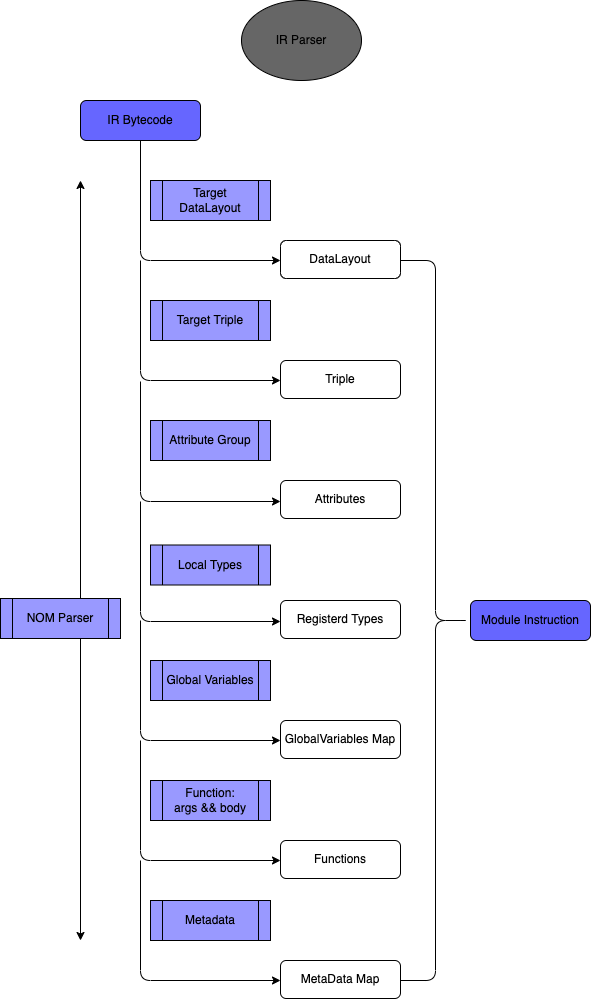
\includegraphics[width=0.6\textwidth]{ola-lang-backend-parser.jpg}
    \caption{ola-lang backend parser pipeline}
    \label{fig:ola-lang-backend-parser}
\end{figure}
\end{itemize}